\documentclass[border=10pt]{standalone}
\usepackage{amsmath}
\usepackage{tikz}
\usetikzlibrary{arrows.meta, calc}

\definecolor{inputcol}{HTML}{4FC3F7}    % light blue — patches
\definecolor{hiddencol}{HTML}{AB47BC}   % purple
\definecolor{attncol}{HTML}{FFA726}     % orange — query patch
\definecolor{winA}{HTML}{B2DFDB}        % window tint A
\definecolor{winB}{HTML}{C5CAE9}        % window tint B

\begin{document}
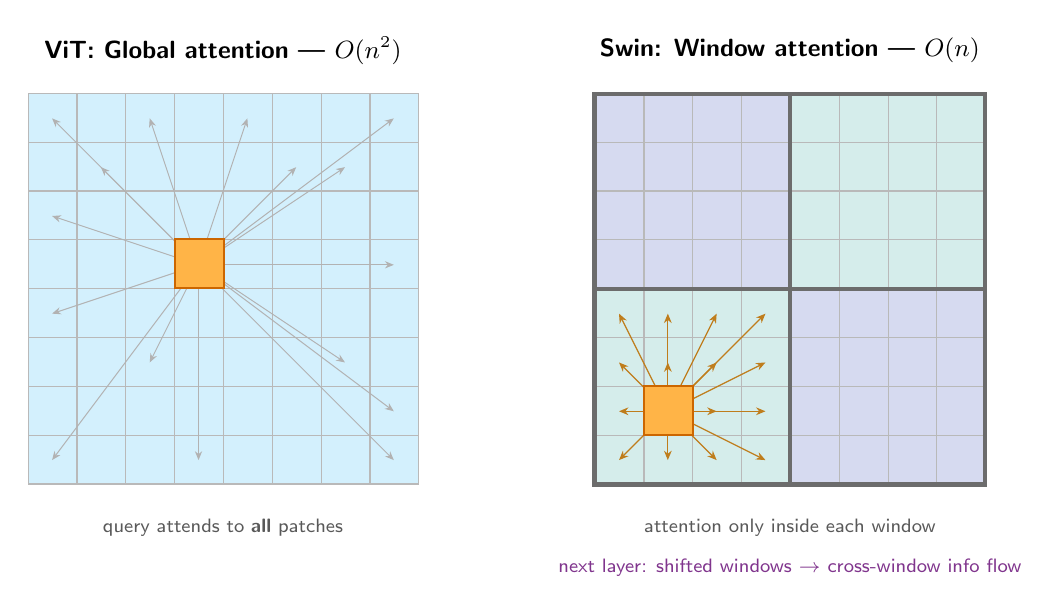
\begin{tikzpicture}[
    cell/.style={draw=gray!55, line width=0.4pt, minimum size=0.62cm,
                 inner sep=0pt, anchor=south west},
    query/.style={cell, fill=attncol!85, draw=orange!80!black, line width=0.7pt},
    attnline/.style={-{Stealth[length=3.2pt, width=2.6pt]},
                     line width=0.35pt, gray!60},
    locline/.style={-{Stealth[length=3.4pt, width=2.8pt]},
                    line width=0.45pt, attncol!75!black},
    title/.style={font=\sffamily\bfseries\small, align=center},
    annot/.style={font=\sffamily\scriptsize, text=gray!70!black, align=center},
  ]

  \def\cs{0.62}   % cell size

  % =========================================================
  %  LEFT PANEL — ViT global attention
  % =========================================================
  \begin{scope}[shift={(0,0)}]
    % grid of patches
    \foreach \i in {0,...,7}{
      \foreach \j in {0,...,7}{
        \node[cell, fill=inputcol!25] at (\i*\cs, \j*\cs) {};
      }
    }
    % query patch near center -> (col 3, row 4) -> centre coord
    \coordinate (qL) at (3*\cs+0.5*\cs, 4*\cs+0.5*\cs);
    \node[query] at (3*\cs, 4*\cs) {};

    % global attention: fan out to representative patches everywhere
    \foreach \tc/\tr in {0/0, 0/3, 0/7, 3/0, 7/0, 7/4, 7/7, 4/7, 0/5,
                         2/2, 6/2, 5/6, 1/6, 6/6, 2/7, 7/1}{
      \draw[attnline] (qL) -- (\tc*\cs+0.5*\cs, \tr*\cs+0.5*\cs);
    }
    % redraw query on top so it stays visible
    \node[query] at (3*\cs, 4*\cs) {};

    % title
    \node[title] at (4*\cs, 8*\cs+0.55) {ViT: Global attention --- $O(n^2)$};
    \node[annot] at (4*\cs, -0.55)
      {query attends to \textbf{all} patches};
  \end{scope}

  % =========================================================
  %  RIGHT PANEL — Swin window attention
  % =========================================================
  \begin{scope}[shift={(7.2,0)}]
    % windows: 2x2 windows of 4x4, alternating tint
    \foreach \i in {0,...,7}{
      \foreach \j in {0,...,7}{
        \pgfmathtruncatemacro{\wx}{\i<4 ? 0 : 1}
        \pgfmathtruncatemacro{\wy}{\j<4 ? 0 : 1}
        \pgfmathtruncatemacro{\parity}{mod(\wx+\wy,2)}
        \ifnum\parity=0
          \node[cell, fill=winA!55] at (\i*\cs, \j*\cs) {};
        \else
          \node[cell, fill=winB!70] at (\i*\cs, \j*\cs) {};
        \fi
      }
    }

    % query inside lower-left window: (col 1, row 1)
    \coordinate (qR) at (1*\cs+0.5*\cs, 1*\cs+0.5*\cs);
    \node[query] at (1*\cs, 1*\cs) {};

    % attends ONLY within its own 4x4 window (cols 0-3, rows 0-3)
    \foreach \tc in {0,...,3}{
      \foreach \tr in {0,...,3}{
        \ifnum\tc=1 \ifnum\tr=1 \else
          \draw[locline] (qR) -- (\tc*\cs+0.5*\cs, \tr*\cs+0.5*\cs);
        \fi\else
          \draw[locline] (qR) -- (\tc*\cs+0.5*\cs, \tr*\cs+0.5*\cs);
        \fi
      }
    }
    \node[query] at (1*\cs, 1*\cs) {};

    % thick window borders
    \draw[line width=1.6pt, gray!85!black]
      (0,0) rectangle (8*\cs, 8*\cs);
    \draw[line width=1.6pt, gray!85!black]
      (4*\cs,0) -- (4*\cs,8*\cs);
    \draw[line width=1.6pt, gray!85!black]
      (0,4*\cs) -- (8*\cs,4*\cs);

    % title
    \node[title] at (4*\cs, 8*\cs+0.55) {Swin: Window attention --- $O(n)$};
    \node[annot] at (4*\cs, -0.55)
      {attention only inside each window};
    \node[annot, text=hiddencol!75!black] at (4*\cs, -1.05)
      {next layer: shifted windows $\rightarrow$ cross-window info flow};
  \end{scope}

\end{tikzpicture}
\end{document}
